\documentclass[11pt,a4paper]{article}
% Shared preamble for the VORB3-SP1 white paper and yellow paper.
\usepackage[T1]{fontenc}
\usepackage[utf8]{inputenc}
\usepackage{lmodern}
\usepackage{amsmath,amssymb,amsthm,mathtools}
\usepackage{booktabs}
\usepackage{longtable}
\usepackage{array}
\usepackage{tabularx}
\usepackage{enumitem}
\usepackage{graphicx}
\usepackage{xcolor}
\usepackage{tikz}
\usetikzlibrary{arrows.meta,positioning,fit,calc,shapes.geometric}
\usepackage{algorithm}
\usepackage{algorithmic}
\usepackage{listings}
\usepackage{caption}
\usepackage{subcaption}
\usepackage{fancyhdr}
\usepackage{microtype}
\usepackage{setspace}
\usepackage{siunitx}
\usepackage[hidelinks]{hyperref}

\definecolor{vorb3blue}{HTML}{1F4E79}
\definecolor{vorb3gray}{HTML}{F2F4F7}
\definecolor{vorb3green}{HTML}{2E6B4F}
\definecolor{vorb3red}{HTML}{8B1E1E}

\hypersetup{
  colorlinks=true,
  linkcolor=vorb3blue,
  citecolor=vorb3blue,
  urlcolor=vorb3blue,
  pdftitle={VORB3-SP1},
  pdfauthor={VORB3 Project},
  pdfsubject={Compact post-quantum signatures},
  pdfkeywords={post-quantum cryptography, VOLEitH, QuickSilver, Rain-SP1, GGM, BLAKE3}
}

\setlength{\parindent}{0pt}
\setlength{\parskip}{0.45em}
\setstretch{1.08}
\setlist[itemize]{topsep=0.35em,itemsep=0.15em,parsep=0.1em}
\setlist[enumerate]{topsep=0.35em,itemsep=0.15em,parsep=0.1em}

\newtheorem{theorem}{Theorem}[section]
\newtheorem{lemma}[theorem]{Lemma}
\newtheorem{proposition}[theorem]{Proposition}
\newtheorem{corollary}[theorem]{Corollary}
\newtheorem{definition}[theorem]{Definition}
\newtheorem{assumption}[theorem]{Assumption}
\theoremstyle{remark}
\newtheorem{remark}[theorem]{Remark}

\newcommand{\F}[1]{\mathbb{F}_{2^{#1}}}
\newcommand{\Fp}{\mathbb{F}}
\newcommand{\bits}{b}
\newcommand{\Fbytes}{F}
\newcommand{\Trees}{T}
\newcommand{\Rounds}{R}
\newcommand{\Gates}{G}
\newcommand{\WH}{\mathsf{WH512}}
\newcommand{\BLAKE}{\mathsf{BLAKE3}}
\newcommand{\KDF}{\mathsf{KDF}}
\newcommand{\Rain}{\mathsf{RainSP1}}
\newcommand{\Gen}{\mathsf{Gen}}
\newcommand{\Sign}{\mathsf{Sign}}
\newcommand{\Verify}{\mathsf{Verify}}
\newcommand{\negl}{\mathsf{negl}}
\newcommand{\Adv}{\mathcal{A}}
\newcommand{\Chal}{\mathcal{C}}
\newcommand{\concat}{\,\|\,}
\newcommand{\xor}{\oplus}
\newcommand{\inv}{^{-1}}
\newcommand{\ceil}[1]{\left\lceil #1 \right\rceil}
\newcommand{\floor}[1]{\left\lfloor #1 \right\rfloor}
\newcommand{\bigO}{\mathcal{O}}
\newcommand{\poly}{\mathsf{poly}}
\newcommand{\ppt}{\mathsf{PPT}}
\newcommand{\sk}{\mathsf{sk}}
\newcommand{\pk}{\mathsf{pk}}
\newcommand{\ct}{\mathsf{ct}}
\newcommand{\pt}{\mathsf{pt}}
\newcommand{\salt}{\mathsf{salt}}
\newcommand{\master}{\mathsf{master}}
\newcommand{\htwo}{h_2}
\newcommand{\com}{\mathsf{com}}
\newcommand{\copath}{\mathsf{copath}}
\newcommand{\outtag}{\mathsf{out\_tag}}
\newcommand{\U}{\mathsf{U}}
\newcommand{\V}{\mathsf{V}}
\newcommand{\Azero}{A_0}
\newcommand{\Aone}{A_1}
\newcommand{\B}{B}
\newcommand{\qstar}{q^\ast}
\newcommand{\ustar}{u^\ast}
\newcommand{\vstar}{v^\ast}
\newcommand{\verify}{\mathsf{verify}}
\newcommand{\vecu}{\mathbf{u}}
\newcommand{\vecw}{\mathbf{w}}
\newcommand{\vecq}{\mathbf{q}}
\newcommand{\vecv}{\mathbf{v}}

\lstset{
  basicstyle=\ttfamily\small,
  breaklines=true,
  columns=fullflexible,
  frame=single,
  rulecolor=\color{vorb3gray},
  backgroundcolor=\color{vorb3gray},
  keepspaces=true,
  showstringspaces=false,
  captionpos=b
}

\pagestyle{fancy}
\fancyhf{}
\fancyhead[L]{\small VORB3-SP1}
\fancyhead[R]{\small\thepage}
\renewcommand{\headrulewidth}{0.4pt}
\fancyfoot[C]{\small Local evidence only --- not an external audit}

\newcommand{\disclaimerbox}[1]{%
  \begin{center}
  \fcolorbox{vorb3red}{vorb3gray}{%
    \begin{minipage}{0.94\linewidth}
    \small\textbf{Security status.} #1
    \end{minipage}}
  \end{center}
}

\newcommand{\doccontrol}[1]{%
  \begin{center}
  \small
  \begin{tabular}{@{}ll@{}}
  \toprule
  Document & #1\\
  Project & VORB3-SP1\\
  Version & 1.3.0\\
  Date & 27 November 2026\\
  Status & Local evidence; no external audit\\
  License & GPL-3.0-or-later\\
  \bottomrule
  \end{tabular}
  \end{center}
}

\hypersetup{pdftitle={VORB3-SP1 Academic White Paper},pdfsubject={Compact post-quantum signatures from Rain-SP1, GGM, and QuickSilver},pdfkeywords={post-quantum signatures, VOLEitH, QuickSilver, Rain-SP1, GGM, BLAKE3}}

\begin{document}

\begin{titlepage}
\centering
\vspace*{2.2cm}
{\color{vorb3blue}\rule{\linewidth}{1.2pt}}\\[0.8cm]
{\Huge\bfseries VORB3-SP1}\\[0.35cm]
{\LARGE A Compact Post-Quantum Signature Scheme\\[0.15cm]
from Rain-SP1, GGM Commitments, and QuickSilver}\\[0.8cm]
{\Large Academic White Paper}\\[0.5cm]
{\color{vorb3blue}\rule{\linewidth}{1.2pt}}\\[1.2cm]

{\large VORB3 Project}\\[0.3cm]
{\large 27 November 2026}\\[0.3cm]
{\large Version 1.3.0}\\[1.0cm]

\doccontrol{Academic White Paper}

\vfill
\begin{minipage}{0.9\linewidth}
\small
\textbf{Abstract.}
We present VORB3-SP1, a compact post-quantum signature design built from a
new inversion-based one-way function (Rain-SP1), a GGM/Merkle vector
commitment, and a QuickSilver-style VOLEitH proof system. The scheme is
implemented in safe Rust as a \texttt{no\_std} library with no allocator, no
runtime dependencies, and a forbidden-unsafe policy. Three parameter profiles
are specified: the frozen SP-288/35 profile with 13,672-byte signatures and a
conservative $\approx$140-bit quantum floor, and two compact NIST-tier packs,
SP-160/32 (Level 1+, 7,976 bytes) and SP-224/32 (Level 3+, 10,296 bytes).
This paper explains the design, the algebraic and proof-system equations, the
security argument and its explicit assumptions, the implementation and
constant-time engineering, the local assurance campaign, and the limitations
of the current evidence. The scheme is a candidate implementation, not an
externally audited or certified product.
\end{minipage}

\vspace{0.7cm}
{\small\textbf{Keywords:} post-quantum signatures, VOLEitH, QuickSilver,
Rain-SP1, GGM, Merkle commitments, BLAKE3, constant-time implementation,
binary fields.}
\end{titlepage}

\disclaimerbox{This white paper describes a locally verified research and
release candidate. It is not a proof of computational security, not an
external audit, and not a NIST/FIPS certification. All quantitative security
figures are conservative accounting targets or bounded local evidence, not
unconditional guarantees.}

\tableofcontents
\newpage

\section{Introduction}

\subsection{Motivation}

Post-quantum signature deployment is constrained by three interacting
requirements: signature size, verification cost, and confidence in the
implementation. Hash-based signatures have a mature security story but large
signatures; lattice signatures are compact and fast but rely on structured
assumptions and complex sampling; code-based and multivariate schemes have
different trade-offs. VORB3-SP1 explores a fourth point in the design space:
a VOLEitH/QuickSilver-style proof of a purpose-built inversion-based one-way
function, with a GGM/Merkle commitment supplying the hidden VOLE
correlations.

The project has four engineering goals:

\begin{enumerate}
  \item \textbf{Compactness.} Keep signatures in the single-digit to low
        double-digit kilobyte range while retaining a conservative
        post-quantum floor.
  \item \textbf{Portability.} Ship a \texttt{no\_std}, heap-free Rust library
        with zero runtime dependencies and no unsafe code.
  \item \textbf{Reproducibility.} Freeze equations, byte layouts, domain
        labels, and known-answer tests so that an independent Python model and
        the Rust implementation can be compared byte for byte.
  \item \textbf{Evidence discipline.} Separate what is proved, what is tested,
        and what is assumed. Do not round up a security estimate into a
        certification claim.
\end{enumerate}

\subsection{Contributions}

This paper makes the following contributions:

\begin{itemize}
  \item A complete specification of the VORB3-SP1 signature scheme over
        binary fields, including key generation, hedged signing, streaming
        GGM/Merkle reconstruction, the VOLE wire map, the zero-safe inversion
        gadget, the batched QuickSilver check, and the public-output tag.
  \item A profile ladder with a frozen SP-288/35 default and two compact
        NIST-tier packs, all sharing the same equations and differing only in
        field size, tree count, and serialized sizes.
  \item A conservative F-33 union-bound accounting that identifies the
        256-bit field as insufficient for an honest 128-bit quantum claim and
        selects 288 bits for the default profile.
  \item An implementation strategy for safe Rust: fixed-size arrays, masked
        arithmetic, no secret-dependent indexing, explicit zeroization,
        streaming tree reconstruction, and a 32 KiB internal stack target.
  \item A local assurance campaign covering KATs, model differentials,
        structured attacks, bit-flip sweeps, fuzzing, mutation, Kani helpers,
        ASan, Miri, coverage, cross-runtime execution, timing measurements,
        and reproducible builds.
  \item A documented set of open problems: full symbolic verification of
        sign/verify, a formal multi-round Rain-SP1 proof, a full QuickSilver
        soundness/ZK proof for this exact circuit, hardware side-channel
        measurement, and external review.
\end{itemize}

\subsection{Status and scope}

The current release line is v1.3.0. The default SP-288/35 profile was frozen
in v1.0.0; the compact packs were introduced in v1.1.0 and v1.2.0 and their
field arithmetic was optimized in v1.3.0 without changing the wire format or
KATs. The library is a candidate implementation. The words ``secure'',
``certified'', and ``audited'' are used only in their precise, limited sense
in this document.

This paper is explanatory. The normative sources are the frozen protocol
specification, the wire-binding table, the implementation, and the frozen
KATs. If this paper and those sources disagree, the frozen sources win.

\subsection{Organization}

Section~\ref{sec:background} reviews the cryptographic background.
Section~\ref{sec:prelim} fixes notation and definitions.
Section~\ref{sec:protocol} gives the protocol overview.
Section~\ref{sec:rain} specifies Rain-SP1.
Section~\ref{sec:vole} defines the VOLE correlation and wire map.
Section~\ref{sec:quicksilver} presents the QuickSilver proof.
Section~\ref{sec:security} gives the security argument and its assumptions.
Section~\ref{sec:impl} describes the implementation.
Section~\ref{sec:evaluation} reports the local evidence.
Section~\ref{sec:discussion} discusses limitations and deployment.
Section~\ref{sec:conclusion} concludes.
The appendices record domain labels, KAT hashes, parameter tables, and the
evidence inventory.

\section{Background and related work}
\label{sec:background}

\subsection{Post-quantum signatures}

A signature scheme is a triple of algorithms $(\Gen,\Sign,\Verify)$ with
correctness and unforgeability requirements. Post-quantum candidates replace
the number-theoretic assumptions of RSA, DSA, and ECDSA with assumptions that
are believed to resist quantum adversaries. The main families are hash-based,
lattice-based, code-based, multivariate, and proof-of-knowledge-based
constructions. VORB3-SP1 belongs to the last family: the signature is a
non-interactive proof of knowledge of a secret witness, made non-interactive
with Fiat--Shamir.

The design uses a VOLEitH-style commitment: the prover and verifier obtain
correlated VOLE shares from hidden leaves of an all-but-one GGM/Merkle
commitment. The proof system is QuickSilver, which proves multiplication
relations over a field using a batched MAC check. The one-way function is
Rain-SP1, a new inversion-based construction with field-linear diffusion.

\subsection{VOLEitH and QuickSilver}

VOLEitH makes VOLE-based zero-knowledge proofs transparent by replacing a
trusted setup with an all-but-one vector commitment. The verifier obtains one
share of a VOLE correlation for each hidden leaf; the prover knows the other
share. The commitment hides the prover's shares and binds the verifier's
shares.

QuickSilver proves arithmetic circuits over a field with a small number of
field elements. For a multiplication gate $(a,b,c)$ with $c=a\cdot b$, the
prover and verifier hold additive shares of the wires and a MAC key $\delta$.
The prover sends masked values, and the verifier checks a batched equation.
The batched check is sound with error proportional to the number of gates
divided by the field size, under the standard VOLE/QuickSilver assumptions.

VORB3-SP1 instantiates these ideas with a 60-gate circuit: four gates per
Rain round for 15 rounds. The circuit has 31 secret wires, one mask leaf, and
a public-output tag. The GGM commitment supplies 32 hidden leaves (31 wires
plus the mask) at the protocol minimum.

\subsection{GGM and Merkle commitments}

A GGM tree expands a short root seed into $2^d$ pseudorandom leaves using a
length-doubling PRG. A Merkle tree commits to the leaves with a collision-
resistant hash. Opening one leaf requires the leaf value and $d$ sibling
nodes; the verifier recomputes the root. Hiding one leaf and opening the rest
gives an all-but-one commitment: the verifier learns all opened leaves, while
the hidden leaf remains secret.

VORB3-SP1 uses depth $d=8$ (256 leaves per tree). The default profile has
$T=35$ trees: 31 secret wires, one mask tree, and three unused challenge
trees that remain committed. The compact packs use the protocol minimum
$T=32$. The hidden leaf index in tree $j$ is derived from byte $j$ of the
64-byte challenge $\htwo$.

\subsection{Rain-SP1}

Rain-SP1 is an inversion-based one-way function over a binary field. Each
round adds a secret key and a public constant, applies field inversion with
$0^{-1}=0$, and multiplies by a public nonzero field constant. The scalar
multiplication is field-linear, so it is free in the QuickSilver proof; this
is the key difference from the original Rain design with a binary MDS matrix,
which a field-VOLE verifier cannot apply to its MAC shares.

Fifteen rounds give 31 secret wires: one for the secret key, 15 inversion
outputs, and 15 zero-selector bits. The mask tree supplies the 32nd hidden
leaf. This is the reason for the protocol constraint $T\ge 2R+2$.

\subsection{BLAKE3 and WH512}

BLAKE3 is a fast, parallelizable cryptographic hash with extendable output.
VORB3-SP1 uses BLAKE3-256 for domain-separated derive-key expansion and keyed
hashing. Because a 256-bit chaining state does not by itself give a 256-bit
collision bound, the protocol uses WH512, a 64-byte construction:
\begin{align*}
\WH(x)={}&\BLAKE_{\mathrm{derive}}(x;\texttt{VORB3-WH512-A-V1})\\
        &\concat\BLAKE_{\mathrm{derive}}(x;\texttt{VORB3-WH512-B-V1}).
\end{align*}
Under the independent-domain-instance assumption, WH512 has the generic
512-bit collision bound: 256-bit classical and approximately 170-bit quantum.
WH512 is used for salts, leaf commitments, Merkle nodes, roots, public-key
hashes, and the transcript state.

\section{Preliminaries}
\label{sec:prelim}

\subsection{Notation}

Let $\F{b}$ denote the binary field with $2^b$ elements, represented in a
polynomial basis. Field addition is bitwise XOR. Let $\Fbytes=b/8$ be the
canonical byte length of a field element; all field elements in the wire
format are little-endian. Let $\xor$ denote XOR and $\concat$ denote
concatenation. For a byte string $x$, $|x|$ is its length. A function
$\epsilon(\lambda)$ is negligible if it is smaller than every inverse
polynomial for all sufficiently large $\lambda$.

We write $\mathcal{A}$ for an adversary, $\Chal$ for a challenger, and
$\negl$ for a negligible function. PPT means probabilistic polynomial time.

\subsection{Signature syntax}

\begin{definition}[Signature scheme]
A signature scheme consists of three algorithms:
\begin{itemize}
  \item $\Gen(1^\lambda)\to(\pk,\sk)$ is randomized key generation;
  \item $\Sign(\sk,m)\to\sigma$ is randomized (or hedged) signing;
  \item $\Verify(\pk,m,\sigma)\to\{0,1\}$ is deterministic verification.
\end{itemize}
Correctness requires $\Verify(\pk,m,\Sign(\sk,m))=1$ for every honestly
generated key pair and every message $m$.
\end{definition}

\begin{definition}[SUF-CMA, informal]
A signature scheme is strongly unforgeable under chosen-message attack if
every PPT adversary with access to a signing oracle cannot produce a valid
signature on a message that was not queried, nor a new valid signature on a
queried message, with non-negligible probability.
\end{definition}

VORB3-SP1 targets SUF-CMA at a conservative 128-bit quantum / 256-bit
classical floor. The target is a design floor, not a certificate.

\subsection{Binary fields}

For the frozen default profile, the field is
\[
\F{288}=\Fp_2[x]/(x^{288}+x^{11}+x^{10}+x+1).
\]
The compact profiles use
\begin{align*}
\F{160}&=\Fp_2[x]/(x^{160}+x^5+x^3+x^2+1),\\
\F{224}&=\Fp_2[x]/(x^{224}+x^9+x^8+x^3+1).
\end{align*}
All three polynomials are irreducible over $\Fp_2$; this is checked locally
with SymPy and recorded in the evidence set. Inversion is defined by
$a^{-1}=a^{2^b-2}$ for $a\ne0$, and $0^{-1}=0$.

\subsection{Transcript}

The transcript is a 64-byte state initialized to
\[
\WH(\texttt{VORB3-TRANSCRIPT-INIT-V1}).
\]
Absorb is length-framed:
\begin{align*}
\mathsf{state}\gets{}&
\WH(\texttt{VORB3-TRANSCRIPT-ABSORB-V1}\concat\mathsf{state}\\
&\concat\mathsf{u64le}(|\ell|)\concat\ell
\concat\mathsf{u64le}(|d|)\concat d).
\end{align*}
Squeeze produces $n$ bytes, then ratchets:
\begin{align*}
\mathsf{out}={}&
\WH(\texttt{VORB3-TRANSCRIPT-SQUEEZE-V1}\concat\mathsf{state}\\
&\concat\mathsf{u64le}(|\ell|)\concat\ell
\concat\mathsf{u64le}(n))[:n],\\
\mathsf{state}\gets{}&
\WH(\texttt{VORB3-TRANSCRIPT-RATCHET-V1}\concat\mathsf{state}\\
&\concat\mathsf{u64le}(n)\concat\mathsf{out}).
\end{align*}
The 512-bit state avoids the 256-bit ratchet collision cap. The signing
schedule absorbs \texttt{PK}, \texttt{SALT}, \texttt{MSG}, and
\texttt{ROOTS}, then squeezes \texttt{DELTA}, \texttt{CHI}, and \texttt{H2}.

\subsection{GGM commitment}

A GGM tree with depth $d=8$ has $2^8=256$ leaves. For tree $j$, the root
seed is derived from the master seed. Each internal node expands to two child
seeds with a domain-separated BLAKE3 derive-key call. The leaf share is a
nonzero field element; the leaf commitment is a WH512 hash of the tree index,
leaf index, salt, public-key hash, and leaf share. Internal nodes hash their
children; the root is the level-0 node hash. The copath contains the eight
sibling seeds from level 8 to level 1.

\section{The VORB3-SP1 protocol}
\label{sec:protocol}

\begin{figure}[ht]
\centering
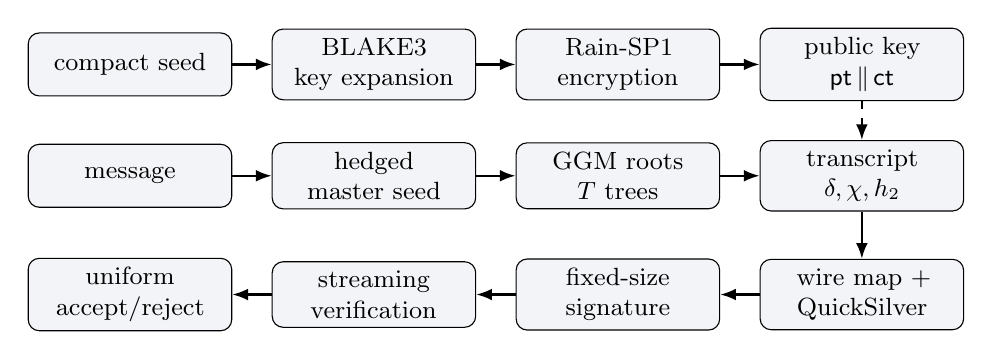
\begin{tikzpicture}[
  font=\small,
  node distance=6mm and 5mm,
  box/.style={draw, rounded corners, align=center, fill=vorb3gray,
              minimum height=8mm, text width=2.35cm},
  arr/.style={-{Latex[length=2mm]}, thick}
]
\node[box] (seed) {compact seed};
\node[box, right=of seed] (key) {BLAKE3\\ key expansion};
\node[box, right=of key] (rain) {Rain-SP1\\ encryption};
\node[box, right=of rain] (pk) {public key\\ $\pt\concat\ct$};
\node[box, below=of seed] (msg) {message};
\node[box, right=of msg] (master) {hedged\\ master seed};
\node[box, right=of master] (roots) {GGM roots\\ $\Trees$ trees};
\node[box, right=of roots] (trans) {transcript\\ $\delta,\chi,\htwo$};
\node[box, below=of trans] (proof) {wire map +\\ QuickSilver};
\node[box, left=of proof] (sig) {fixed-size\\ signature};
\node[box, left=of sig] (verify) {streaming\\ verification};
\node[box, left=of verify] (accept) {uniform\\ accept/reject};
\draw[arr] (seed) -- (key);
\draw[arr] (key) -- (rain);
\draw[arr] (rain) -- (pk);
\draw[arr] (msg) -- (master);
\draw[arr] (master) -- (roots);
\draw[arr] (roots) -- (trans);
\draw[arr] (trans) -- (proof);
\draw[arr] (proof) -- (sig);
\draw[arr] (sig) -- (verify);
\draw[arr] (verify) -- (accept);
\draw[arr, dashed] (pk) -- (trans);
\end{tikzpicture}
\caption{End-to-end flow. The public key is derived from the seed; signing
binds the roots, message, and public key through the transcript; verification
reconstructs roots and checks the MAC, gate, mask, and output-tag equations.}
\label{fig:flow}
\end{figure}

\subsection{Profiles}

\begin{table}[ht]
\centering
\small
\caption{Shipped profiles. $F$ is the field width in bytes, $T$ the tree
count. The conservative floor is the minimum of the component floors; it is
not a certification.}
\label{tab:profiles}
\resizebox{\linewidth}{!}{%
\begin{tabular}{@{}lcccccccc@{}}
\toprule
Profile & Feature & Field & $T$ & Rounds & Signature & Public key & Seed & Floor (q/c) \\
\midrule
SP-288/35 & default & $\F{288}$ & 35 & 15 & 13,672 & 72 & 36 & $\approx$140 / 256 \\
SP-160/32 & \texttt{nist1} & $\F{160}$ & 32 & 15 & 7,976 & 40 & 20 & $\approx$76.5 / 153.1 \\
SP-224/32 & \texttt{nist3} & $\F{224}$ & 32 & 15 & 10,296 & 56 & 28 & $\approx$108.5 / 217.1 \\
\bottomrule
\end{tabular}}
\end{table}

The public key is $2\Fbytes$ bytes, the compact seed is $\Fbytes$ bytes, and
the expanded secret is $3\Fbytes$ bytes. The signature length is
\begin{equation}
\mathsf{SIG}=128+34\Fbytes+\Trees(8\Fbytes+64).
\label{eq:siglen}
\end{equation}
The first 128 bytes are the salt and $\htwo$; $34\Fbytes$ covers the 31
wire responses, $U$, $V$, and the output tag; $\Trees\cdot8\Fbytes$ is the
copath; $\Trees\cdot64$ is the hidden-leaf commitments.

\subsection{Key generation}

Given a seed $s\in\{0,1\}^{\Fbytes}$,
\begin{align}
\sk &= \mathsf{nonzero}(\mathsf{field}(\KDF_\Fbytes(\texttt{VORB3-KEYGEN-SK-V1},s))),\\
\pt &= \mathsf{nonzero}(\mathsf{field}(\KDF_\Fbytes(\texttt{VORB3-KEYGEN-PT-V1},s))),\\
\ct &= \Rain(\sk,\pt),\\
\pk &= \mathsf{bytes}(\pt)\concat\mathsf{bytes}(\ct).
\end{align}
The nonzero map replaces zero by one in constant time. Public-key parsing
rejects $\pt=0$ or $\ct=0$. The expanded secret contains $\sk$, $\pt$, and
the seed; it is zeroized on drop.

\subsection{Signing}

Signing is hedged. The caller supplies 32 bytes of entropy. The all-zero
value is a test/KAT input and is not appropriate for production. The master
seed is
\[
\master=\KDF_\Fbytes(\texttt{VORB3-HEDGED-V1},
\mathsf{bytes}(\sk)\concat\pk\concat\mathsf{u64le}(|m|)\concat m\concat e),
\]
and the salt is
$\salt=\WH(\texttt{VORB3-SALT-V1}\concat\master)$.

The signer then performs two passes over the GGM trees. Pass A derives the
$\Trees$ roots. The transcript absorbs $\pk$, $\salt$, $m$, and the roots,
and squeezes $\delta$, $\chi$, and $\htwo$. Pass B re-expands each tree,
extracts the copath for the hidden index, and computes the hidden leaf share
and commitment. The Rain witness and ciphertext are computed, the 31 secret
wires are filled, and the 60 QuickSilver gates are batched with $\chi$. The
mask leaf produces $(U,V)$; the output tag is the MAC of $\ct$. The signature
is serialized in the fixed order of Section~\ref{sec:wire}.

\begin{algorithm}[ht]
\small
\caption{$\Sign(\sk,m,e)$ (informative)}
\label{alg:sign}
\begin{algorithmic}[1]
\REQUIRE expanded secret $\sk$, message $m$, entropy $e\in\{0,1\}^{256}$
\ENSURE signature $\sigma$ or error
\STATE validate $\sk\ne0$, $\pt\ne0$, $\ct\ne0$
\STATE $\pk\gets\pt\concat\ct$; $\mathsf{pkh}\gets\WH(\texttt{VORB3-PK-HASH-V1}\concat\pk)$
\STATE $\master\gets\KDF(\cdot)$; $\salt\gets\WH(\texttt{VORB3-SALT-V1}\concat\master)$
\FOR{$j=0$ to $\Trees-1$}
  \STATE derive root seed; expand tree; compute leaf commitments and root
\ENDFOR
\STATE transcript absorbs PK, SALT, MSG, ROOTS
\STATE $(\delta,\chi,\htwo)\gets$ squeeze DELTA, CHI, H2
\FOR{$j=0$ to $\Trees-1$}
  \STATE re-expand tree $j$; extract copath at index $\htwo[j]$
  \STATE compute hidden share $u_j$ and commitment $\com_j$; set $q_j\gets\com_j[0:\Fbytes]$
\ENDFOR
\STATE compute Rain witness $(x_r,y_r,b_r,s_r)$ and $\ct$
\STATE build 31 wires and masks $d_i=u_i\xor w_i$
\STATE compute 60 gate pairs; batch with $\chi$
\STATE compute $\U=\Azero\xor\vstar$, $\V=\Aone\xor\ustar$
\STATE $\outtag\gets v_{\ct}$
\STATE serialize $\salt,\htwo,d,U,V,\outtag,\copath,\com$
\STATE wipe master, seeds, shares, witness, and intermediates
\RETURN $\sigma$
\end{algorithmic}
\end{algorithm}

\subsection{Wire format}
\label{sec:wire}

All field elements are $\Fbytes$ bytes, little-endian; hashes and roots are
64 bytes; seeds are $\Fbytes$ bytes. The signature is exactly
$128+34\Fbytes+\Trees(8\Fbytes+64)$ bytes and has no trailing bytes:
64 bytes of salt, 64 bytes of $\htwo$, $31\Fbytes$ of wire responses,
$\Fbytes$ each for $U$, $V$, and $\outtag$, $\Trees\cdot8\Fbytes$ of
copaths, and $\Trees\cdot64$ bytes of hidden-leaf commitments. The exact
byte offsets and the copath/hidden-commitment order are normative in the
yellow paper and in \texttt{docs/WIRE-BINDING.md}.

\subsection{Verification}

Verification rejects a wrong length before parsing. It reconstructs each
Merkle root from the hidden commitment and copath, recomputes the transcript,
and checks $\htwo$ in constant time. It then recomputes the verifier MACs
$q_i'=q_i\xor d_i\delta$, evaluates the linear wires and all gate values
$B_i$, batches with $\chi$, and checks the mask equation and the public-output
tag. All signature-content failures collapse to one uniform error.

\begin{algorithm}[ht]
\small
\caption{$\Verify(\pk,m,\sigma)$ (informative)}
\label{alg:verify}
\begin{algorithmic}[1]
\REQUIRE public key $\pk$, message $m$, signature bytes $\sigma$
\ENSURE accept/reject
\STATE reject if $|\sigma|\ne\mathsf{SIG}$ or $\pk$ has a zero component
\STATE parse $\salt,\htwo,d,U,V,\outtag,\copath,\com$
\FOR{$j=0$ to $\Trees-1$}
  \STATE reconstruct root from $\com_j$ and $\copath_j$
\ENDFOR
\STATE recompute transcript with PK, SALT, MSG, ROOTS
\STATE squeeze $(\delta',\chi',\htwo')$; check $\htwo'=\htwo$ in constant time
\FOR{each of the 31 wires}
  \STATE $q_i'\gets q_i\xor d_i\delta$
\ENDFOR
\STATE compute $q$ for all linear wires and $B_i$ for all gates
\STATE batch with $\chi$; check $\B\xor\qstar=\U\xor\V\delta$
\STATE check $q_{\ct}=\outtag\xor\ct\delta$
\STATE return one uniform decision
\end{algorithmic}
\end{algorithm}

\section{Rain-SP1}
\label{sec:rain}

\subsection{Design rationale}

Rain-SP1 is an inversion-based one-way function with a public field-linear
diffusion layer. It replaces the binary MDS matrix of the original Rain design
because a field-VOLE verifier cannot apply an arbitrary binary matrix to its
MAC shares. Multiplication by a nonzero field constant is $\F{b}$-linear and
therefore free in the proof.

The key schedule is minimal: the same secret key is added in every round and
once at the output. The 30 public constants prevent pure slide symmetry.
Fifteen rounds are the security-margin baseline and the maximum that fits the
31-wire/tree-32 layout. The round count is not reduced to fit a smaller
signature.

\subsection{Constants}

For a profile with field size $b$, let
\[
\mathsf{tag}=\texttt{VORB3-RAIN}b\texttt{-SP}.
\]
For $r=0,\ldots,14$,
\begin{align}
K_r&=\mathsf{nonzero}(\mathsf{field}(\KDF_\Fbytes(
  \mathsf{tag}\concat\texttt{-K}r\texttt{-V1},
  \mathsf{tag}\concat\texttt{-CONSTANTS-V1}))),\\
c_r&=\mathsf{nonzero}(\mathsf{field}(\KDF_\Fbytes(
  \mathsf{tag}\concat\texttt{-C}r\texttt{-V1},
  \mathsf{tag}\concat\texttt{-CONSTANTS-V1}))).
\end{align}
All constants are public, deterministic, nonzero, and distinct. They are
checked in the constant tests and are not secret-dependent.

\subsection{Encryption}

\begin{algorithm}[ht]
\small
\caption{$\Rain(\sk,\pt)$}
\label{alg:rain}
\begin{algorithmic}[1]
\REQUIRE $\sk,\pt\in\F{b}$, both nonzero
\ENSURE $\ct\in\F{b}$ and witness $(x_r,y_r,b_r,s_r)_{r=0}^{14}$
\STATE $s\gets\pt$
\FOR{$r=0$ to $14$}
  \STATE $x_r\gets s\xor\sk\xor K_r$
  \STATE $y_r\gets x_r\inv$ \COMMENT{$0\inv=0$}
  \STATE $b_r\gets 1$ if $x_r=0$, else $0$
  \STATE $s\gets c_r\cdot y_r$
\ENDFOR
\STATE $\ct\gets s\xor\sk$
\RETURN $(\ct,(x_r,y_r,b_r,s_r))$
\end{algorithmic}
\end{algorithm}

\subsection{Zero-safe inversion gadget}

The proof cannot use the cubic relation $x^2y\xor x=0$ because it does not
force $y=0$ when $x=0$. VORB3-SP1 uses the four equations
\begin{align}
b\cdot b&=b,\label{eq:g1}\\
b\cdot x&=0,\label{eq:g2}\\
b\cdot y&=0,\label{eq:g3}\\
x\cdot y&=1\xor b.\label{eq:g4}
\end{align}

\begin{lemma}[Zero-safe gadget]
The system~\eqref{eq:g1}--\eqref{eq:g4} has exactly the two honest solutions:
$(b,x,y)=(1,0,0)$ when $x=0$, and $(b,x,y)=(0,x,x\inv)$ when $x\ne0$.
\end{lemma}
\begin{proof}
Equation~\eqref{eq:g1} forces $b\in\{0,1\}$. If $b=1$, then $x=0$ by
\eqref{eq:g2}, $y=0$ by \eqref{eq:g3}, and \eqref{eq:g4} gives $0=0$. If
$b=0$, then $xy=1$ by \eqref{eq:g4}, so $x\ne0$ and $y=x\inv$. The cases are
exhaustive.
\end{proof}

The selector bit $b_r$ is a secret witness and is masked by the proof. It does
not reveal whether an intermediate state is zero.

\subsection{Differential analysis}

For even $b$, inversion over $\F{b}$ is 4-differentially uniform:
\[
\max_{a\ne0,b}\Pr_{x}\left[x\inv\xor(x\xor a)\inv=b\right]=\frac{4}{2^b}.
\]
The claim follows by clearing denominators: for $a,b\ne0$, the equation
$1/x\xor1/(x\xor a)=b$ gives a quadratic with at most two roots, and the two
boundary points $x=0$ and $x=a$ add at most two more. Affine input/output maps
do not change the differential distribution. Hence each Rain round has
maximum differential probability at most $4/2^b$.

For $R$ rounds, the crude composition bound is
\[
\max\mathsf{DP}\le 2^{b(R-1)}\left(\frac{4}{2^b}\right)^R
=\frac{4^R}{2^b}=2^{2R-b}.
\]
For $b=288$ and $R=15$, this is $2^{-258}$. The bound is conservative and
weakens with $R$; it is a valid upper bound, not a multi-round security proof.
No full-width differential trail search has been completed.

\subsection{Linear and algebraic notes}

The inversion permutation has a large single-round Walsh coefficient; for
toy fields the measured pattern is consistent with a correlation of
approximately $2^{-(b/2-1)}$. The multi-round correlation-matrix bound is
vacuous after summing over $2^b$ intermediate masks, so no useful multi-round
linear bound is claimed. The algebraic degree of inversion is $b-1$; toy
experiments show degree saturation at the maximum immediately. A full-width
interpolation or Gr\"obner attack is far outside the local budget. These are
arguments and limitations, not proofs.

\begin{assumption}[Rain-SP1 security]
Rain-SP1 with 15 or more rounds resists key recovery, algebraic, differential,
and linear attacks at the profile's target field size. This is a
cryptanalytic assumption and a release gate, not a theorem.
\end{assumption}

\section{VOLE correlation and wire assignment}
\label{sec:vole}

\subsection{Correlation}

For a hidden leaf in tree $j$, the prover holds a leaf share $u$, and the
verifier holds
\[
q=\mathsf{field}(\com[0:\Fbytes]).
\]
The prover's tag is
\[
v=q\xor u\cdot\delta.
\]
After the prover sends the opening $d=u\xor w$ for a wire value $w$, the
verifier computes
\[
q'=q\xor d\cdot\delta=v\xor w\cdot\delta.
\]
The verifier knows $q,d,\delta,q'$; the prover knows $u,v,w$. The witness $w$
is hidden by the one-time pad $u$, and $v$ is random.

\subsection{Wire map}

\begin{table}[ht]
\centering
\small
\caption{Fixed wire map for the default profile. The compact profiles have the
same wire indices; only field sizes change.}
\label{tab:wires}
\begin{tabular}{@{}cll@{}}
\toprule
Wire(s) & Tree(s) & Meaning \\
\midrule
0 & 0 & secret key $\sk$ \\
1--15 & 1--15 & inversion outputs $y_0,\ldots,y_{14}$ \\
16--30 & 16--30 & zero selectors $b_0,\ldots,b_{14}$ \\
-- & 31 & mask tuple $(u^\ast,v^\ast)$ \\
\bottomrule
\end{tabular}
\end{table}

\subsection{Linear wires and MACs}

The public/linear wires are assigned as follows:
\begin{align}
\pt &: w=\pt,\quad q=\pt\cdot\delta,\quad v=0,\\
0 &: w=0,\quad q=0,\quad v=0,\\
1 &: w=1,\quad q=\delta,\quad v=0,\\
K_r &: w=K_r,\quad q=K_r\cdot\delta,\quad v=0,\\
x_r &: w=s_{r-1}\xor\sk\xor K_r,\quad
      q=q_s\xor q_{\sk}\xor K_r\cdot\delta,\quad
      v=v_s\xor v_{\sk},\\
s_r &: w=c_r y_r,\quad q=c_r q_{y_r},\quad v=c_r v_{y_r},\\
1\xor b_r &: w=1\xor b_r,\quad q=\delta\xor q_{b_r},\quad v=v_{b_r}.
\end{align}
The initial $s_0=\pt$ has $q=\pt\cdot\delta$, $v=0$. The final ciphertext
$\ct=s_{15}\xor\sk$ has
$q_{\ct}=q_s\xor q_{\sk}$ and $v_{\ct}=v_s\xor v_{\sk}$. The prover sends
$\outtag=v_{\ct}$; the verifier checks
\[
q_{\ct}=\outtag\xor\ct\cdot\delta.
\]

\section{QuickSilver proof}
\label{sec:quicksilver}

\subsection{Gate equations}

For each round, in order, the four gates are
\begin{align}
b_r\cdot b_r&=b_r,\\
b_r\cdot x_r&=0,\\
b_r\cdot y_r&=0,\\
x_r\cdot y_r&=1\xor b_r.
\end{align}
For a gate $(a,b,c)$, the prover computes
\begin{align}
\Azero &= v_a v_b,\\
\Aone  &= w_a v_b\xor w_b v_a\xor v_c.
\end{align}
The verifier computes
\[
\B=q_a q_b\xor q_c\delta.
\]
If the gate is correct, $\B=\Azero\xor\Aone\delta$.

\subsection{Batching}

Let $\chi$ be the transcript challenge and $G=60$ for 15 rounds. The prover
computes
\[
\Azero=\bigoplus_{i=0}^{G-1}A_{0,i}\chi^i,\qquad
\Aone=\bigoplus_{i=0}^{G-1}A_{1,i}\chi^i,
\]
and the verifier computes
\[
\B=\bigoplus_{i=0}^{G-1}\B_i\chi^i.
\]

\subsection{Mask}

The mask tree (tree 31) gives $(u^\ast,v^\ast)$ with verifier share
$q^\ast=\com_{31}[0:\Fbytes]$ and
\[
v^\ast=q^\ast\xor u^\ast\cdot\delta.
\]
The prover sends
\[
\U=\Azero\xor v^\ast,\qquad \V=\Aone\xor u^\ast.
\]
The verifier checks
\[
\B\xor q^\ast=\U\xor\V\cdot\delta.
\]
This is a one-time pad: the verifier knows $q^\ast$ but not $u^\ast,v^\ast$.

\subsection{Soundness sketch}

For a wrong multiplication gate, $\B\xor\Azero\xor\Aone\delta$ is a nonzero
polynomial in $\delta$ of degree at most two. For a fixed cheating prover, a
random $\delta$ passes with probability at most $2/|\F{b}|$. Batching with a
random $\chi$ reduces the 60 checks to one; the conservative union bound is
$G\cdot2/|\F{b}|$. The exact published QuickSilver bound may be tighter, but
the security case deliberately uses the conservative bound until a tighter
argument is formalized.

The selector equations force $y=\mathrm{inv}(x)$ for every round. The output
tag forces the public ciphertext. The VOLEitH all-but-one commitment binds the
hidden leaf values under the WH512 collision assumption. The Fiat--Shamir
transcript binds the roots and hidden indices.

\subsection{Zero-knowledge sketch}

The wire opening $d_i=u_i\xor w_i$ is a one-time pad; $u_i$ is a secret hidden
leaf share. The verifier's MAC $q_i'=v_i\xor w_i\delta$ is randomized by
$v_i$. The witness values $\sk,y_r,b_r$ never appear in the signature. The
batched $\Azero,\Aone$ are masked by the independent mask leaf; the public
output tag is a MAC tag, not a witness value. A simulator can sample the
verifier's shares and the masked values. A full simulation argument for this
exact circuit is future work; the present document records only the sketch.

\section{Security analysis}
\label{sec:security}

\subsection{Assumptions}

\begin{assumption}[Rain-SP1]
Rain-SP1 with 15 rounds is a one-way function and resists the stated
cryptanalytic attacks at the profile field size.
\end{assumption}

\begin{assumption}[BLAKE3/WH512]
BLAKE3 behaves as a random oracle/PRF for independent domain instances, and
WH512 has the generic 512-bit collision bound under the independent-instance
assumption.
\end{assumption}

\begin{assumption}[VOLEitH/QuickSilver]
The all-but-one GGM commitment and the QuickSilver batch check retain their
standard soundness and zero-knowledge properties in this instantiation.
\end{assumption}

\begin{assumption}[Fiat--Shamir]
The transcript is a random oracle and Fiat--Shamir is sound for the
commitment-then-challenge schedule used here.
\end{assumption}

\subsection{Completeness}

\begin{theorem}[Completeness]
If the signer follows the protocol and all primitives are correct, then
$\Verify(\pk,m,\Sign(\sk,m,e))=1$ for every message $m$ and entropy $e$.
\end{theorem}
\begin{proof}[Proof sketch]
The honest selector $b_r=1$ iff $x_r=0$ satisfies the four gadget equations.
The linear wires have MAC/tag pairs derived from the secret wires, so the MAC
relations hold by linearity. The gate equations hold term-by-term, hence the
batched equation holds. The mask tuple is a valid one-time pad, and the public
output tag is the MAC of $\ct$. The GGM roots and transcript are recomputed
identically. The Python model asserts every relation for the toy and full
profiles, and the Rust KAT matches it byte for byte.
\end{proof}

\subsection{Soundness}

\begin{proposition}[Conditional soundness]
Under Assumptions 1--4, a cheating prover that produces a verifying signature
for a message not signed by the honest signer implies either a break of
Rain-SP1, a collision in WH512, a break of the VOLEitH/QuickSilver
instantiation, or a Fiat--Shamir forgery. The conservative per-signature
soundness error is at most
\[
\epsilon_{\mathrm{sound}}
\le \frac{2G}{|\F{b}|}+\epsilon_{\mathrm{FS}}+\epsilon_{\mathrm{commit}}.
\]
\end{proposition}
\begin{proof}[Proof sketch]
The gadget equations force the selector and inversion relation. The batched
gate check fails a wrong multiplication with probability at most $2/|\F{b}|$
per gate; the union bound gives $2G/|\F{b}|$. The wire MACs bind the opened
wires to the hidden commitments; a mismatch implies a commitment collision or
a VOLEitH break. The transcript binds the roots and indices; a forgery with a
different message or roots implies a Fiat--Shamir break or a collision. The
model and KAT exercise completeness, not soundness; the bound is a
conservative accounting argument, not a machine-checked proof.
\end{proof}

\subsection{SUF-CMA argument}

The signature is a non-interactive proof of knowledge of a secret witness for
the Rain-SP1 public relation, bound to the message by the transcript. Under
the assumptions above, a SUF-CMA forger either extracts a witness (breaking
Rain-SP1 one-wayness), finds a collision in the commitment or transcript
(binding), or breaks the proof system's soundness. The public key is
$\pt\concat\ct$; a forger that changes $\pt$ or $\ct$ must produce a
consistent Rain witness and output tag. The wire openings and mask are
one-time-padded, so they do not reveal the witness. The argument is
conditional and excludes the open items in Section~\ref{sec:limits}.

\subsection{F-33 accounting}

The 256-bit field is insufficient for an honest 128-bit quantum claim under
the conservative union bound. The field-check term is approximately
$b/2-0.5\log_2(2G)$; for $b=256$ and $G=60$ this is about 125 bits. The
project therefore freezes 288 bits for the default profile and uses 160/224
bits only for the explicitly labelled NIST-tier packs.

\begin{table}[ht]
\centering
\small
\caption{Conservative component floors in bits (quantum/classical). The
overall floor is the minimum; it is not a certification.}
\label{tab:floors}
\resizebox{\linewidth}{!}{%
\begin{tabular}{@{}lcccccc@{}}
\toprule
Profile & Field check & Tree challenge & Key & WH512 & Overall & Signature \\
\midrule
SP-288/35 & 140.5 / 281.1 & 140 / 280 & 144 / 288 & 170 / 256 & \textbf{140 / 256} & 13,672 \\
SP-160/32 & 76.5 / 153.1 & 128 / 256 & 80 / 160 & 170 / 256 & \textbf{76.5 / 153.1} & 7,976 \\
SP-224/32 & 108.5 / 217.1 & 128 / 256 & 112 / 224 & 170 / 256 & \textbf{108.5 / 217.1} & 10,296 \\
\bottomrule
\end{tabular}}
\end{table}

\subsection{What is not proved}
\label{sec:limits}

The following are explicitly outside the current evidence:

\begin{itemize}
  \item computational security of Rain-SP1 at full width;
  \item a machine-checked soundness/ZK proof for the exact QuickSilver circuit;
  \item full symbolic Kani verification of sign/verify;
  \item constant-time execution as a formal theorem;
  \item absolute zeroization of compiler temporaries;
  \item a 72-hour fuzz soak;
  \item external audit or NIST certification.
\end{itemize}

\section{Implementation}
\label{sec:impl}

\subsection{Rust architecture}

The shipped crate is \texttt{no\_std}, forbids unsafe code, and has no
third-party runtime dependencies. It uses fixed-size arrays throughout and
does not allocate. The public API exposes:
\begin{itemize}
  \item \texttt{SecretKey}, \texttt{ExpandedSecretKey}, \texttt{PublicKey};
  \item \texttt{Signature}, \texttt{sign}, \texttt{sign\_into},
        \texttt{verify}, \texttt{verify\_bytes};
  \item fixed constants for field, key, and signature lengths;
  \item feature-selected profile constants.
\end{itemize}
Verification failures return one uniform error. The caller supplies 32 bytes
of entropy for signing.

\subsection{Field arithmetic}

The default 288-bit field uses 64-bit limbs, a specialized bit-interleaved
square, a word-level product reduction, and a 16-entry Itoh--Tsujii inversion
chain. The compact profiles use 32-bit limbs and the same high-level strategy:
bit-interleaved squaring, word-level reduction for $b\bmod32=0$, and an
Itoh--Tsujii binary chain. The v1.3.0 optimization reduced compact-field
inversion by roughly 60--70$\times$ and made both compact packs faster to sign
than the baseline. All loops are fixed-count; control flow depends only on
public parameters.

\subsection{Constant-time discipline}

The code uses mask-based selection, fixed iteration counts, and
\texttt{black\_box} barriers. Secret values are never used as array indices or
branch conditions. Verification accumulates checks without an early exit on
signature content. Zeroization is best-effort: owned secret buffers are
wiped on drop and on explicit wipe, with a compiler barrier. The evidence is
statistical and dynamic (dudect, cachegrind, ctgrind, assembly review); it is
not a formal constant-time proof.

\subsection{GGM streaming}

Signing uses two passes over the trees to avoid storing all 35 full trees. The
first pass derives the roots and absorbs them into the transcript. The second
pass re-expands each tree, extracts the copath, and computes the hidden share.
Verification reconstructs each root from the hidden commitment and copath; the
verifier does not re-expand the hidden leaf subtree. The 32 KiB stack target
covers the internal working set; a caller that puts the full signature on the
stack needs a larger budget.

\subsection{Error handling and API}

Wrong signature length, wrong public-key component, invalid MAC, failed
selector checks, and a failed output tag all map to one \texttt{InvalidSignature}
error. A degenerate secret key maps to \texttt{InvalidSecretKey}. Public-key
parsing rejects zero $\pt$ or $\ct$. The API never returns a partial
signature. All fixed-size parsing is checked; no panic, unwrap, or indexing
lints are permitted.

\section{Evaluation}
\label{sec:evaluation}

\subsection{Functional evidence}

The Rust implementation matches the independent Python model for the frozen
KAT and for 28 signature differential cases (0--8192 bytes). The field
differential covers 4,096 random records for each compact field; the default
profile has 512 vectors. Structured tests cover truncation, trailing bytes,
wrong keys, wrong messages, replay, cross-context reuse, component swaps,
duplication, and region damage. The single-bit signature sweep rejects
109,376 default-profile mutations, 63,808 Level 1+ mutations, and 82,368
Level 3+ mutations.

\subsection{Fuzzing and mutation}

The v1.0.0 baseline accumulated 405,581,569 libFuzzer executions with zero
crashes. The v1.3.0 compact-pack campaigns ran 12,310,692 (Level 1+) and
24,575,666 (Level 3+) executions with zero crashes. Targeted mutation found
494 baseline mutants and 427 mutants per compact pack; the compact-pack misses
are 26 expression-equivalent mutants in 21 Z3-checked classes plus three
unobservable \texttt{Drop} wipes.

\subsection{Bounded verification and memory safety}

Kani proves 18 helper harnesses for the default profile and 16 per compact
pack, covering field encoding, additive and multiplicative identities,
constant-time equality/select, zero tests, public-key parsing, signature
length, and wipe helpers. Full symbolic sign/verify is not tractable at the
local budget. ASan passes the full graph. Miri passes the full default
sign+verify KAT and selected field/key primitives under strict provenance and
symbolic alignment for the compact packs. Valgrind memcheck and
\texttt{cargo-careful} complete without reports on the tested paths.

\subsection{Coverage and stack}

Coverage is 100\% of functions and 99.90\% of lines for the default
all-features graph, and 100\% of functions and 99.70\% of lines for each
compact profile. The residual compact-profile lines are guard returns in test
code. The release stack target is 32 KiB for the internal working set on
x86\_64, AArch64, s390x, i686, ppc64, Windows, and WASI; the 64 KiB case covers
the full default signature on the caller's stack.

\subsection{Cross-platform runtime}

KATs and full test graphs pass on AArch64, s390x (big-endian), i686, ppc64
(big-endian), Windows/Wine, and WASI. The library has no runtime dependencies,
so the cross-platform surface is the compiler and \texttt{core}.

\subsection{Performance}

\begin{table}[ht]
\centering
\small
\caption{v1.3.0 release medians, 25 samples per operation, same host.}
\label{tab:perf}
\begin{tabular}{@{}lrrr@{}}
\toprule
Operation & SP-288/35 & Level 1+ & Level 3+ \\
\midrule
Key generation & 266.1 $\mu$s & 74.2 $\mu$s & 151.8 $\mu$s \\
Sign, 32 B & 6.364 ms & 4.855 ms & 5.105 ms \\
Verify, 32 B & 5.676 ms & 4.639 ms & 4.648 ms \\
Sign + verify, 32 B & 12.007 ms & 9.501 ms & 9.834 ms \\
Rain encryption & 257.9 $\mu$s & 69.4 $\mu$s & 146.7 $\mu$s \\
Field multiplication & 712 ns & 216 ns & 409 ns \\
Field squaring & 13.4 ns & 10.5 ns & 11.8 ns \\
Field inversion & 17.36 $\mu$s & 4.43 $\mu$s & 9.40 $\mu$s \\
\bottomrule
\end{tabular}
\end{table}

The compact packs trade a larger field-inversion cost for smaller signatures;
after the v1.3.0 optimization they are faster than the baseline to sign and
verify. GGM/BLAKE3 root derivation is the remaining dominant signing cost
(about 93--96\%). Message hashing scales at roughly 3.1--3.4 ms/MiB for
signing and 2.1--2.2 ms/MiB for verification.

\subsection{Side channels and reproducibility}

Dudect at 50,000 samples passes the $|t|<4.5$ threshold for sign and verify on
all profiles. Cachegrind and assembly review are local evidence, not a formal
constant-time proof. Two clean release builds produce byte-identical rlibs:
\texttt{60e98d9c\ldots} for v1.0.0, \texttt{bc245cdb\ldots} for Level 1+, and
\texttt{cf198c13\ldots} for Level 3+.

\section{Discussion}
\label{sec:discussion}

\subsection{Deployment considerations}

VORB3-SP1 is not a drop-in replacement for a standardized signature scheme.
A deployment must consider:
\begin{itemize}
  \item the absence of external audit and standardized cryptanalysis;
  \item the large signature size relative to lattice schemes;
  \item the need for caller-supplied entropy and secure seed storage;
  \item the 32 KiB internal stack target and the larger caller stack budget
        when the full signature is placed on the stack;
  \item the platform and compiler dependence of side-channel behavior;
  \item the need to select exactly one profile feature and to pin the frozen
        KATs.
\end{itemize}

\subsection{Open problems}

The most important open problems are a full-width Rain-SP1 cryptanalysis, a
machine-checked soundness/ZK proof for the exact circuit, a full symbolic
verification of sign/verify, a 72-hour fuzz soak, hardware side-channel
measurement, Apple runtime coverage, and external review. The project treats
these as release blockers for stronger claims, not as details to be rounded
away.

\subsection{Comparison}

Qualitatively, VORB3-SP1 sits between hash-based signatures (large signatures,
very conservative assumptions) and lattice signatures (compact signatures,
structured assumptions). Its distinguishing feature is the proof-of-knowledge
structure over a purpose-built inversion function, with a transparent GGM
commitment and a field-linear diffusion layer. A quantitative comparison
would require a common security accounting and is outside the scope of this
paper.

\section{Conclusion}
\label{sec:conclusion}

VORB3-SP1 is a compact post-quantum signature design with a fully specified
wire format, an independent executable model, a safe Rust implementation, and
a deep local assurance campaign. The default SP-288/35 profile has a
conservative $\approx$140-bit quantum floor and 13,672-byte signatures. The
NIST-tier packs provide 7,976-byte and 10,296-byte signatures with explicit
floors above their nominal categories. The v1.3.0 compact-field optimization
makes both packs faster to sign and verify than the baseline.

The project is deliberately explicit about what it has not proved. It is a
candidate implementation with local evidence, not an externally audited or
certified product. The next step is independent review and the open
cryptanalytic and formal-verification work listed in
Section~\ref{sec:limits}.

\appendix

\section{Domain labels}

\begin{longtable}{@{}p{0.42\linewidth}p{0.5\linewidth}@{}}
\toprule
Context / label & Purpose \\
\midrule
\endhead
\texttt{VORB3-WH512-A-V1} & WH512 left domain \\
\texttt{VORB3-WH512-B-V1} & WH512 right domain \\
\texttt{VORB3-GGM-EXPAND-V1} & GGM child expansion \\
\texttt{VORB3-KEYGEN-SK-V1} & secret-key derivation \\
\texttt{VORB3-KEYGEN-PT-V1} & plaintext derivation \\
\texttt{VORB3-HEDGED-V1} & hedged master seed \\
\texttt{VORB3-PK-HASH-V1} & public-key hash \\
\texttt{VORB3-TREE-ROOT-V1} & tree root seed \\
\texttt{VORB3-RAIN\{...\}-SP-CONST-V1} & Rain constants seed \\
\texttt{VORB3-RAIN\{...\}-SP-K\{r\}-V1} & round key constants \\
\texttt{VORB3-RAIN\{...\}-SP-C\{r\}-V1} & diffusion constants \\
\texttt{VORB3-SALT-V1} & salt derivation \\
\texttt{VORB3-GGM-LEAF-V1} & leaf commitment \\
\texttt{VORB3-GGM-NODE-V1} & internal node hash \\
\texttt{VORB3-TRANSCRIPT-INIT-V1} & transcript initial state \\
\texttt{VORB3-TRANSCRIPT-ABSORB-V1} & transcript absorb \\
\texttt{VORB3-TRANSCRIPT-SQUEEZE-V1} & transcript squeeze \\
\texttt{VORB3-TRANSCRIPT-RATCHET-V1} & transcript ratchet \\
\bottomrule
\end{longtable}

\section{KAT manifest}

\begin{table}[ht]
\centering
\small
\caption{Frozen KAT SHA-256 digests. The full signature bytes are checked into
\texttt{kat/}.}
\label{tab:kat}
\begin{tabular}{@{}lccc@{}}
\toprule
Profile & Seed SHA-256 & Public key SHA-256 & Signature SHA-256 \\
\midrule
SP-288/35 & \texttt{dd1b0529\ldots} & \texttt{a7b5a252\ldots} & \texttt{c073c7e3\ldots} \\
SP-160/32 & \texttt{88b90539\ldots} & \texttt{7a0756e5\ldots} & \texttt{43dcf2de\ldots} \\
SP-224/32 & \texttt{4248e3fd\ldots} & \texttt{753312d0\ldots} & \texttt{3ad501e1\ldots} \\
\bottomrule
\end{tabular}
\end{table}

The raw seed and public-key bytes for the three profiles are:
\begin{align*}
\text{SP-288/35 seed} &= \texttt{46bc6ad6e6af38f0d15f3f1b56d8e28279cd735231de2a1ca0}\\
&\quad\texttt{abb8dc122d961f4b415421},\\
\text{SP-288/35 pk} &= \texttt{6380aa2d\ldots f255239047395cdb91b7},\\
\text{SP-160/32 seed} &= \texttt{1e4fae52c4eb017ceb51cb1d365d8db45c7d8c79},\\
\text{SP-160/32 pk} &= \texttt{ae858e22\ldots aa8cfdaafb1bcf7d},\\
\text{SP-224/32 seed} &= \texttt{3da55abb2a69d2ff59d0d33955d46c3c}\\
&\quad\texttt{b4cb28d347a88ede82442e5e},\\
\text{SP-224/32 pk} &= \texttt{47218a67\ldots f2842aabadc812319}.
\end{align*}

\section{Parameter and evidence tables}

\begin{table}[ht]
\centering
\small
\caption{Signature length decomposition. Values are bytes.}
\label{tab:sigdecomp}
\begin{tabular}{@{}lrrr@{}}
\toprule
Component & SP-288/35 & Level 1+ & Level 3+ \\
\midrule
Salt + $\htwo$ & 128 & 128 & 128 \\
Wire responses $31F$ & 1,116 & 620 & 868 \\
$U+V+\outtag$ ($3F$) & 108 & 60 & 84 \\
Copaths $T\cdot8F$ & 10,080 & 5,120 & 7,168 \\
Hidden commitments $T\cdot64$ & 2,240 & 2,048 & 2,048 \\
\midrule
Total & 13,672 & 7,976 & 10,296 \\
\bottomrule
\end{tabular}
\end{table}

\begin{table}[ht]
\centering
\small
\caption{Assurance summary. Numbers are local evidence, not a certificate.}
\label{tab:assurance}
\begin{tabular}{@{}lccc@{}}
\toprule
Check & SP-288/35 & Level 1+ & Level 3+ \\
\midrule
KAT + model differential & pass & pass & pass \\
Field differential & 512 vectors & 4,096 & 4,096 \\
Single-bit sweep & 109,376 & 63,808 & 82,368 \\
libFuzzer executions & 405,581,569 & 12,310,692 & 24,575,666 \\
Targeted mutants & 494 & 427 & 427 \\
Kani helpers & 18/18 & 16/16 & 16/16 \\
ASan & pass & pass & pass \\
Miri & full & field+keys & field+keys \\
Coverage lines & 99.90\% & 99.70\% & 99.70\% \\
32 KiB stack & pass & pass & pass \\
Cross-runtime & pass & pass & pass \\
Dudect sign/verify & $-1.383/0.552$ & $-0.317/-0.468$ & $1.460/0.977$ \\
Reproducible rlib & \texttt{60e98d9c\ldots} & \texttt{bc245cdb\ldots} & \texttt{cf198c13\ldots} \\
\bottomrule
\end{tabular}
\end{table}

\begin{thebibliography}{99}

\bibitem{GGM86}
O. Goldreich, S. Goldwasser, and S. Micali.
\newblock How to construct random functions.
\newblock \emph{Journal of the ACM}, 33(4):792--807, 1986.

\bibitem{Merkle87}
R. C. Merkle.
\newblock A digital signature based on a conventional encryption function.
\newblock In \emph{CRYPTO}, 1987.

\bibitem{FS86}
A. Fiat and A. Shamir.
\newblock How to prove yourself: Practical solutions to identification and
signature problems.
\newblock In \emph{CRYPTO}, 1986.

\bibitem{QuickSilver}
C. Baum, L. Braun, C. Delpech de Saint Guilhem, M. Kloo\ss,
E. Orsini, L. Roy, and P. Scholl.
\newblock QuickSilver: Efficient and affordable zero-knowledge proofs for
circuits and polynomials over any field.
\newblock In \emph{ACM CCS}, 2021.

\bibitem{VOLEitH}
C. Baum, C. Delpech de Saint Guilhem, M. Kloo\ss, E. Orsini, and P. Scholl.
\newblock VOLEitH: Making VOLE-based zero-knowledge proofs transparent.
\newblock In \emph{CRYPTO}, 2022.

\bibitem{BLAKE3}
J. O'Connor, J.-P. Aumasson, S. Neves, and Z. Wilcox-O'Hearn.
\newblock BLAKE3: One function, fast everywhere.
\newblock 2020. \url{https://blake3.io}.

\bibitem{NISTPQ}
National Institute of Standards and Technology.
\newblock Post-quantum cryptography standardization.
\newblock \url{https://csrc.nist.gov/projects/post-quantum-cryptography}.

\end{thebibliography}

\end{document}
